\section{Problem Formulation}\label{sec:pro}
In this part, we first formally define the \textit{fidelity-optimal sampling problem} in Section~\ref{sec:def} and then show that it is NP-hard to solve the problem exactly in Section~\ref{sec:hard}.

\begin{figure}
	\centering
	\small
	\begin{tabular}{cc}
        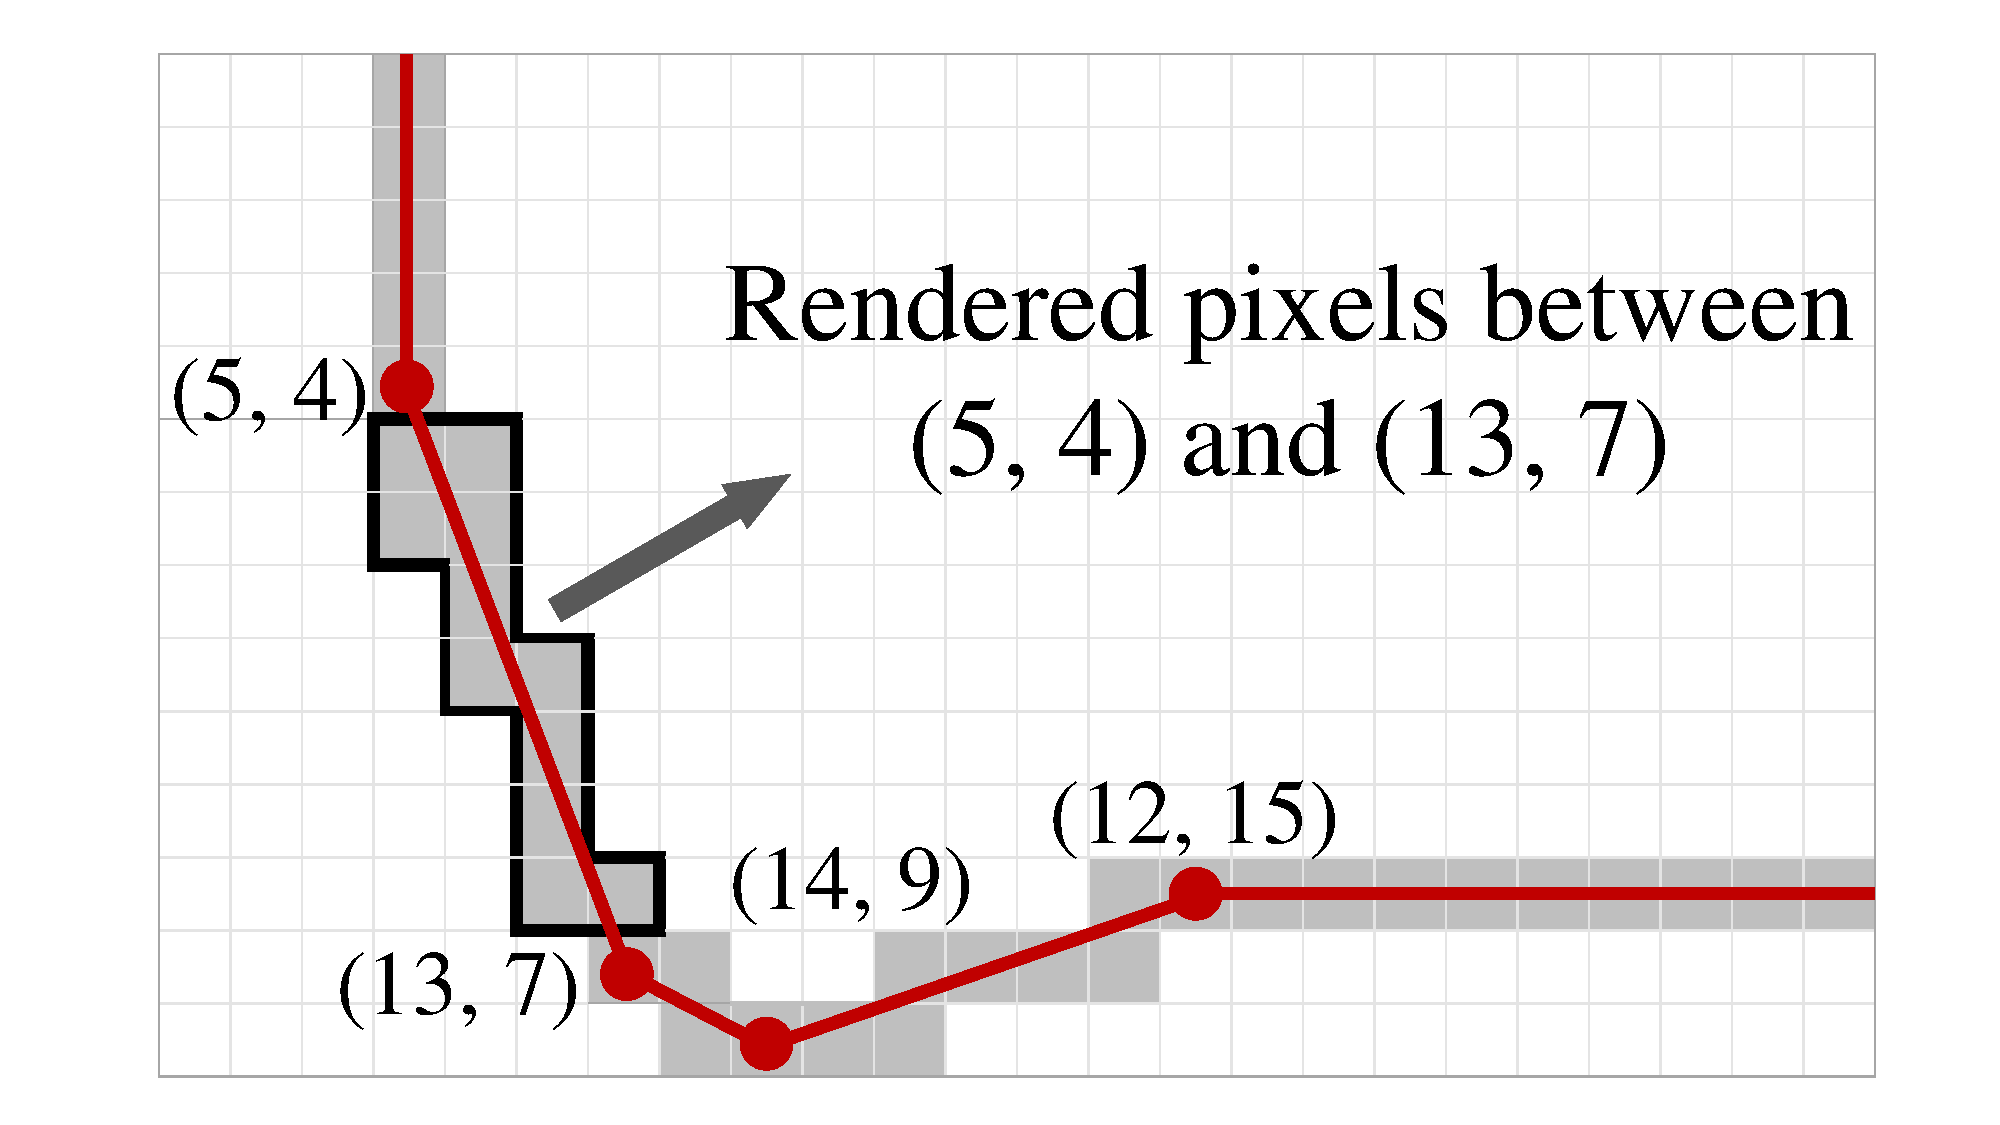
\includegraphics[width=0.43\columnwidth]{pictures/problemsolveing/RenderedPixels}
		&
        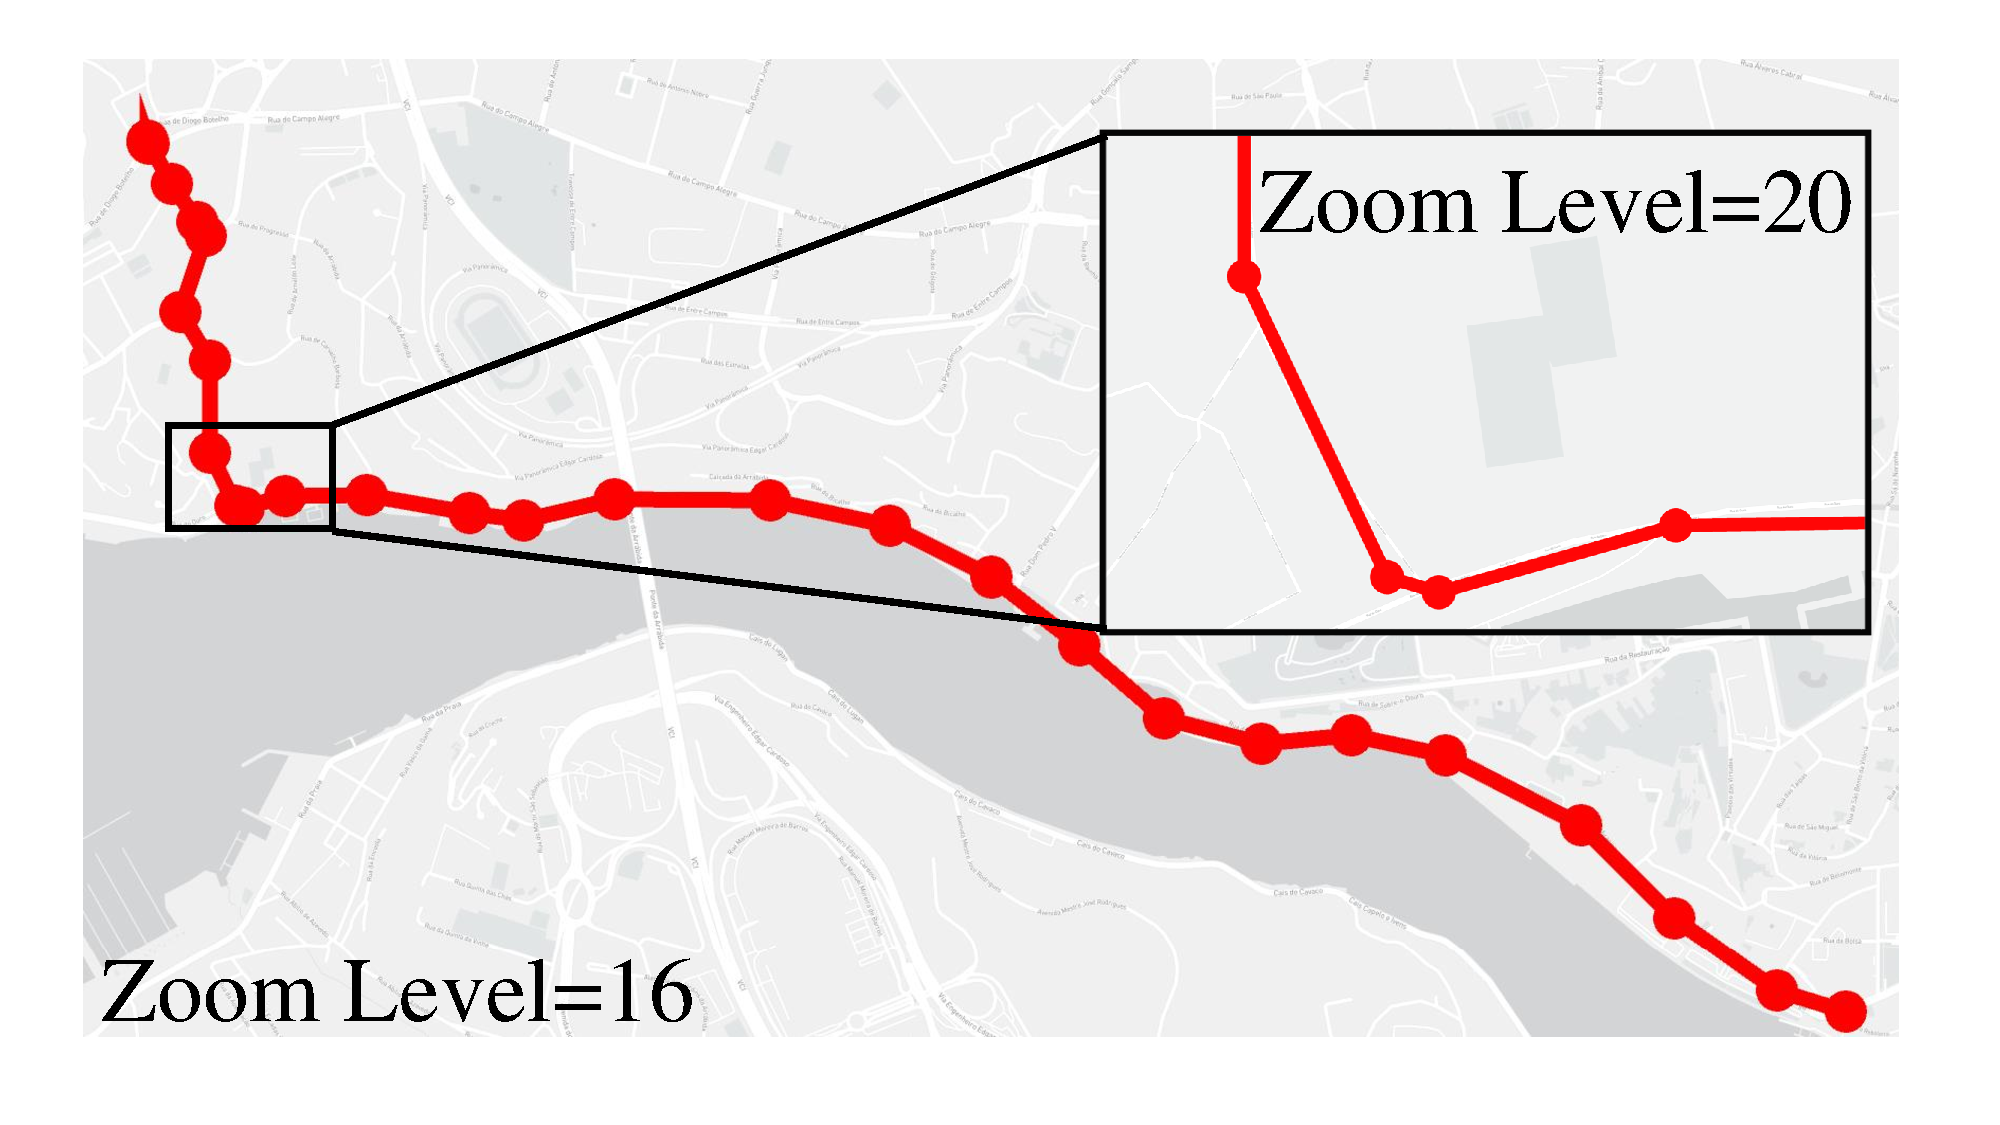
\includegraphics[width=0.48\columnwidth]{pictures/problemsolveing/TrajZoomIn}		
		\\
		(A) Line-based visualization
		&
        (B) Zoom levels
	\end{tabular}
	\vspace{-4mm}
	\caption{Illustration of line-based trajectory visualization.} \label{fig:line}
	\vspace{-6mm}
\end{figure}


\subsection{Problem Definition}\label{sec:def}


We motivate our definition of the \textit{fidelity loss function} by introducing how line-based trajectory visualization works. As introduced earlier, a trajectory contains a sequence of 2-dimensional locations. Given an empty canvas (i.e., the screen of a displaying device) with pixels indexed by horizontal and vertical coordinates (i.e., $x$ and $y$), line-based trajectory visualization connects consecutive locations in each trajectory with polylines and marks the pixels passed by these polylines (with a color different from the background). As shown in Figure~\ref{fig:line}(A), the result of line-based trajectory visualization can be regarded as a 2-dimensional array of boolean variables with 1 indicting a pixel has been marked. Alternatively, we can treat a visualization result $\mathcal{V}$ as a set that contains all marked pixels. This observation leads to the following definition of the fidelity loss function
\begin{equation}\label{eqref:loss}
loss(\mathcal{V}, \mathcal{V}')=\frac{|\mathcal{V}-\mathcal{V}'|}{|\mathcal{V}|},
\end{equation}
in which $|.|$ measures the cardinality of a set, and set $\mathcal{V}^\star=\mathcal{V}-\mathcal{V}'$ contains all distinct elements between $\mathcal{V}$ and $\mathcal{V}'$. We use $loss(\mathcal{V}, \mathcal{V}')$ to measure the fidelity loss of a visualization result $\mathcal{V}'$ compared to the ground-truth visualization $\mathcal{V}$. This definition matches human visual perception as it is essentially the ratio of different pixels in two visualization results. Thus, the approximate visualization $\mathcal{V}'$ will look similar to $\mathcal{V}$ if $loss(\mathcal{V}, \mathcal{V}')$ is small.


Given the fidelity loss function, we are ready to define the fidelity-optimal sampling problem. Denote the set of all trajectories in a dataset as $\mathcal{T}$ and a subset of $\mathcal{T}$ (which contains some sampled trajectories) as $\mathcal{R}$. With a slight abuse of the notation, we use $V(\mathcal{S})$ to denote the visualization results derived from a set $\mathcal{S}$ of trajectories.

\begin{problem}[Fidelity-optimal sampling problem]\label{prob:def}
	Given a sampling rate $\alpha$, find a set $\mathcal{R}$ that satisfies
	\begin{equation}\label{eq:opp}
	\min_{\mathcal{R} \subseteq \mathcal{T}, |\mathcal{R} | = \alpha \mathcal{T} } loss(V(\mathcal{T}), V(\mathcal{R})).
	\end{equation}
\end{problem}
If there is a solution for the above fidelity-optimal sampling problem, to provide a guaranteed fidelity $loss(V(\mathcal{T}), V(\mathcal{R}))\le \tau$, we can simply use a binary search to find the smallest $\alpha$ under which the visual fidelity requirement holds.

One subtlety is that trajectory visualization needs to work at different \textit{zoom levels} upon user request. For example, Google map~\cite{googlemap} provides a zoom levels from 0 to 20, with level 0 providing the largest visualization range (i.e., the whole world) but the lowest resolution, and level 20 providing the smallest visualization range (e.g., individual building, if available) but the highest resolution. We also provided an illustration of zoom level in Figure~\ref{fig:line}(B). Ideally, we want a sample to be \textit{zoom-level-independent}, providing a consistent fidelity guarantee at different zoom levels. This turns out to be straightforward as trajectory visualization merges several pixels in a high-level result (by pixel-wise $OR$) to obtain a pixel in a lower-level visualization result. The following theorem shows that it suffices to satisfy the fidelity guarantee at the highest zoom level.
\begin{theorem}~\label{the:level}
	Use~$loss(V(\mathcal{T}), V(\mathcal{R}), l)$ to denote the fidelity loss induced by a sample set $\mathcal{R}$ at zoom level $l$, we have~ $loss(V(\mathcal{T}), V(\mathcal{R}), l) \\ \le loss(V(\mathcal{T}), V(\mathcal{R}), l')$ if $l\le l'$, with larger $l$ indicating higher resolution.
\end{theorem}

%\REPORT{
\begin{proof}
	Denote the value of the pixel at location $(x,y)$ for the visualization result of zoom level $l$ as $p^l(x,y)$, which can be either 0 or 1 in line-based trajectory visualization. Recall that pixels of lower zoom levels are obtained by merging pixels from lower zoom levels with pixel-wise OR. Thus, we have $p^l(x,y)=\vee_{(a,b)\in g(x,y,l,l')} \ p^{l'}(a,b)$, in which  $l\le l'$ and $g(x,y,l,l')$ is the set of pixels in the visualization of zoom level $l'$ that are used to determine $p^l(x,y)$ at zoom level $l$. Use $p^l_{V(\mathcal{S})}(x,y)$ to denote the $p^l(x,y)$ induced by a set $\mathcal{S}$ of sample trajectories, we have
	$p^l_{V(\mathcal{T})}(x,y)=p^l_{V(\mathcal{R})}(x,y) \ \text{if} \ \exists (a,b)\in g(x,y) \ \text{~~such that~~} p^{l'}_{V(\mathcal{T})}(x,y)=p^{l'}_{V(\mathcal{R})}(x,y).$ It follows that
	\begin{align} \nonumber
	loss(V(\mathcal{T}),V(\mathcal{R}),l)=   \frac{|V^l(\mathcal{T})-V^l(\mathcal{T})|}{|V^l(\mathcal{T})|}\le \\  \frac{|V^{l'}(\mathcal{T})-V^{l'}(\mathcal{T})|}{|V^{l'}(\mathcal{T})|}=loss(V(\mathcal{T}), V(\mathcal{R}), l').
	\end{align}

\end{proof}
%}

We are aware that lower zoom levels need more coarse-grained visualization and thus the sampling rate at the highest level may be larger than necessary. We left more sophisticated designs, such as re-sampling a sample set or generating multiple sample sets for future work, and consider only sampling for the highest zoom level. As our fidelity loss function considers the entire visible region (i.e., it is a \textit{global fidelity measure}), the visual difference between our sample and the ground-truth visualization may be large for some specific regions, especially when the marked points are sparse in these regions. \textit{Local visual fidelity} can be important for some tasks(e.g., outlier discovery~\cite{feng2010matching,mayorga2013splatterplots}) and we leave it for future work. We want to note that a fidelity-guaranteed sample $\mathcal{R}$ is also \textit{query independent} from the definition of the fidelity loss function, which means $\mathcal{R}$ only needs to be constructed once to answer all queries.

\subsection{Hardness Analysis}\label{sec:hard}
We use $t_i \in \mathcal{T}$ to denote a trajectory in the dataset. According to the working mechanism of line-based trajectory visualization, $t_i$ corresponds to a set of marked pixels on the canvas in the ground-truth visualization and we also use $t_i$ to denote this set of pixels. Thus, we have $V(\mathcal{T}) = \cup_{t_i \in \mathcal{T}} t_i$ and $V(\mathcal{R}) = \cup_{t_i \in \mathcal{R}} t_i$. We can transform Problem~\ref{prob:def} as follows

\begin{align}\label{eqn:obj2} \nonumber
\min_{\oR \subseteq \D, |\oR| = \alpha |\D|}  \frac{|\V(\D) - \V(\oR)|}{|\V(\D)|}  & \Leftrightarrow \min_{\oR \subseteq \D, |\oR| = \alpha |\D|}   - |\V(\oR)| \\ \nonumber
 \Leftrightarrow \max_{\oR \subseteq \D, |\oR| = \alpha |\D|}  |\V(\oR)| &  \Leftrightarrow \max_{\oR \subseteq \D, |\oR| = \alpha |\D|} | \cup_{t_i \in \oR} t_i |
\end{align}

The above transformations use the fact that $V(\mathcal{R}) \subset V(\mathcal{T})$ as $\mathcal{R} \subset \mathcal{T}$, and the ground-truth set $V(\mathcal{T})$ is constant. The last line shows that fidelity-optimal sampling is equivalent to the well-known set cover maximization problem.
Specifically, given an integer $k = \alpha |\D|$, and a collection trajectory pixel set $\D = \{t_1, t_2, \cdots, t_n \}$, set cover maximization finds a subset $\oR \subset \D$ such that $|\oR| \leq k$ and $|\cup_{t_i \in \oR} t_i|$ is maximized. The set cover maximization problem is well-known to be NP-hard~\cite{setcover}.


%It is equivalent to select sized-$k$ trajectory set $\oR$ from $\D$ which $\cup_{\oR_i \in \oR} \oR_i$ is maximized.
%It is a NP-hard problem as we proved in Lemma~\ref{lem:np}.

%\begin{lemma}[NP hard]~\label{lem:np}
%Given a trajectory dataset $\D$ and an integer $k$,
%The sampling-based trajectory visualization problem (see Problem~\ref{prob:def}) is NP-hard.
%\end{lemma}

%We omit the proof of Lemma~\ref{lem:np} as it is a typical set cover maximization problem\footnote{\url{https://en.wikipedia.org/wiki/Maximum_coverage_problem}}, which is a well-known NP-hard problem in literature.

%------------comments by Bo-------------------
%As we analyzed in Section~\ref{sec:intro}, the large-scale (e.g., hundreds of millions GPS points) line-based trajectory visualization problem is very challenging due to the large data size and limited rendering capability of graphics devices.
%To make matters worse, the visualization result of large-scale trajectory dataset suffers visual clutter seriously.
%In this work, we focus on how to visualize large-scale trajectory dataset efficiently and effectively.
%In particular, our objective is to devise a visual fidelity guaranteed sampling method for large trajectory data visualization.
%The major challenges to achieve this goal are:
%(i) how to define visual fidelity theoretically? (ii) how to guarantee the visual fidelity of the sampling-based visualization result?
